%\documentclass[aps,pra,reprint,longbibliography]{revtex4-1}
\documentclass[twocolumn]{article}

\usepackage{geometry}
\geometry{textwidth = 18cm,textheight = 24cm}

%\usepackage{multicol}
\usepackage{cite}
\usepackage{caption}
\usepackage{graphicx}
\usepackage{amsmath}
\usepackage{float}
%\usepackage{amssymb}
\usepackage{textcomp}
\usepackage{lmodern}
\newenvironment{figure_alt}
  {\par\medskip\noindent\minipage{\linewidth}}
  {\endminipage\par\medskip}

\begin{document}
	
	%-------------------- begin header -------------------%
	\centerline{\LARGE Fluxonic processing}
	\vspace{0.5em}
	\centerline{\LARGE of photonic synapse events}
	\vspace{0.75em}
	\centerline{\large Jeffrey M. Shainline}
	%\vspace{0.75em}
	%\centerline{\large National Institute of Standards and Technology}
	\vspace{0.5em}
	\centerline{\normalsize NIST, Boulder, CO, 80305}
	\vspace{0.5em}
	\centerline{\small \today}
	%-------------------- end header ---------------------%
	
\begin{abstract}

\end{abstract}

\tableofcontents

\section{\label{sec:introduction}Introduction}
	
the dendritic arbor has also be re-envisioned to occur in the electronic domain; fan-out photonic, fan-in electronic	

\begin{figure} 
    \centering{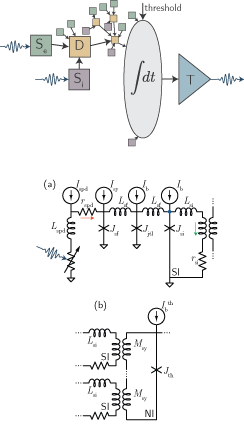
\includegraphics[width=8.6cm]{_1_schematic_and_circuits.png}}
	\captionof{figure}{\label{fig:schematicAndCircuits}Caption.}
\end{figure}

\section{\label{sec:synapse}Photon-to-fluxon transduction at a synapse}

\begin{figure} 
    \centering{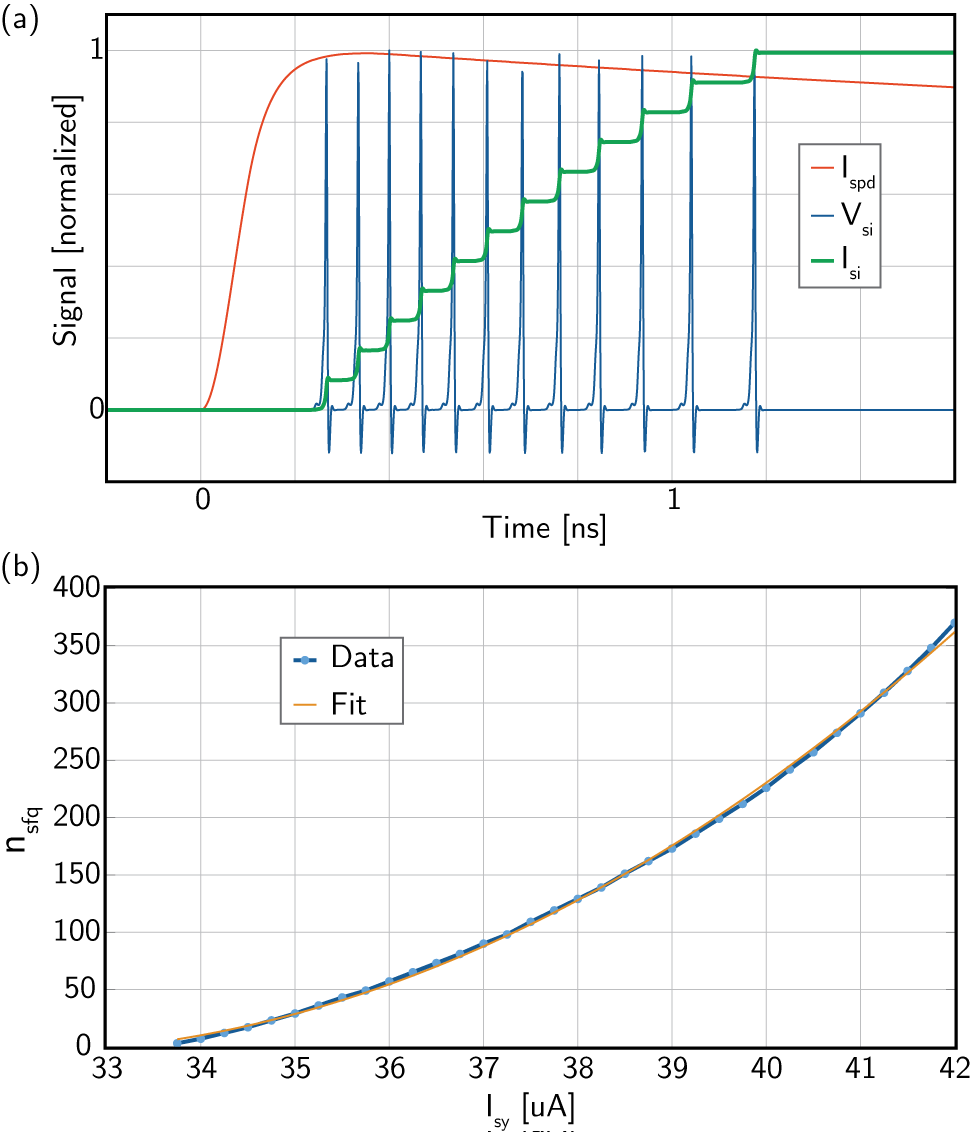
\includegraphics[width=8.6cm]{_2_sffg_basic.png}}
	\captionof{figure}{\label{fig:sffg}Caption.}
\end{figure}

\begin{figure} 
    \centering{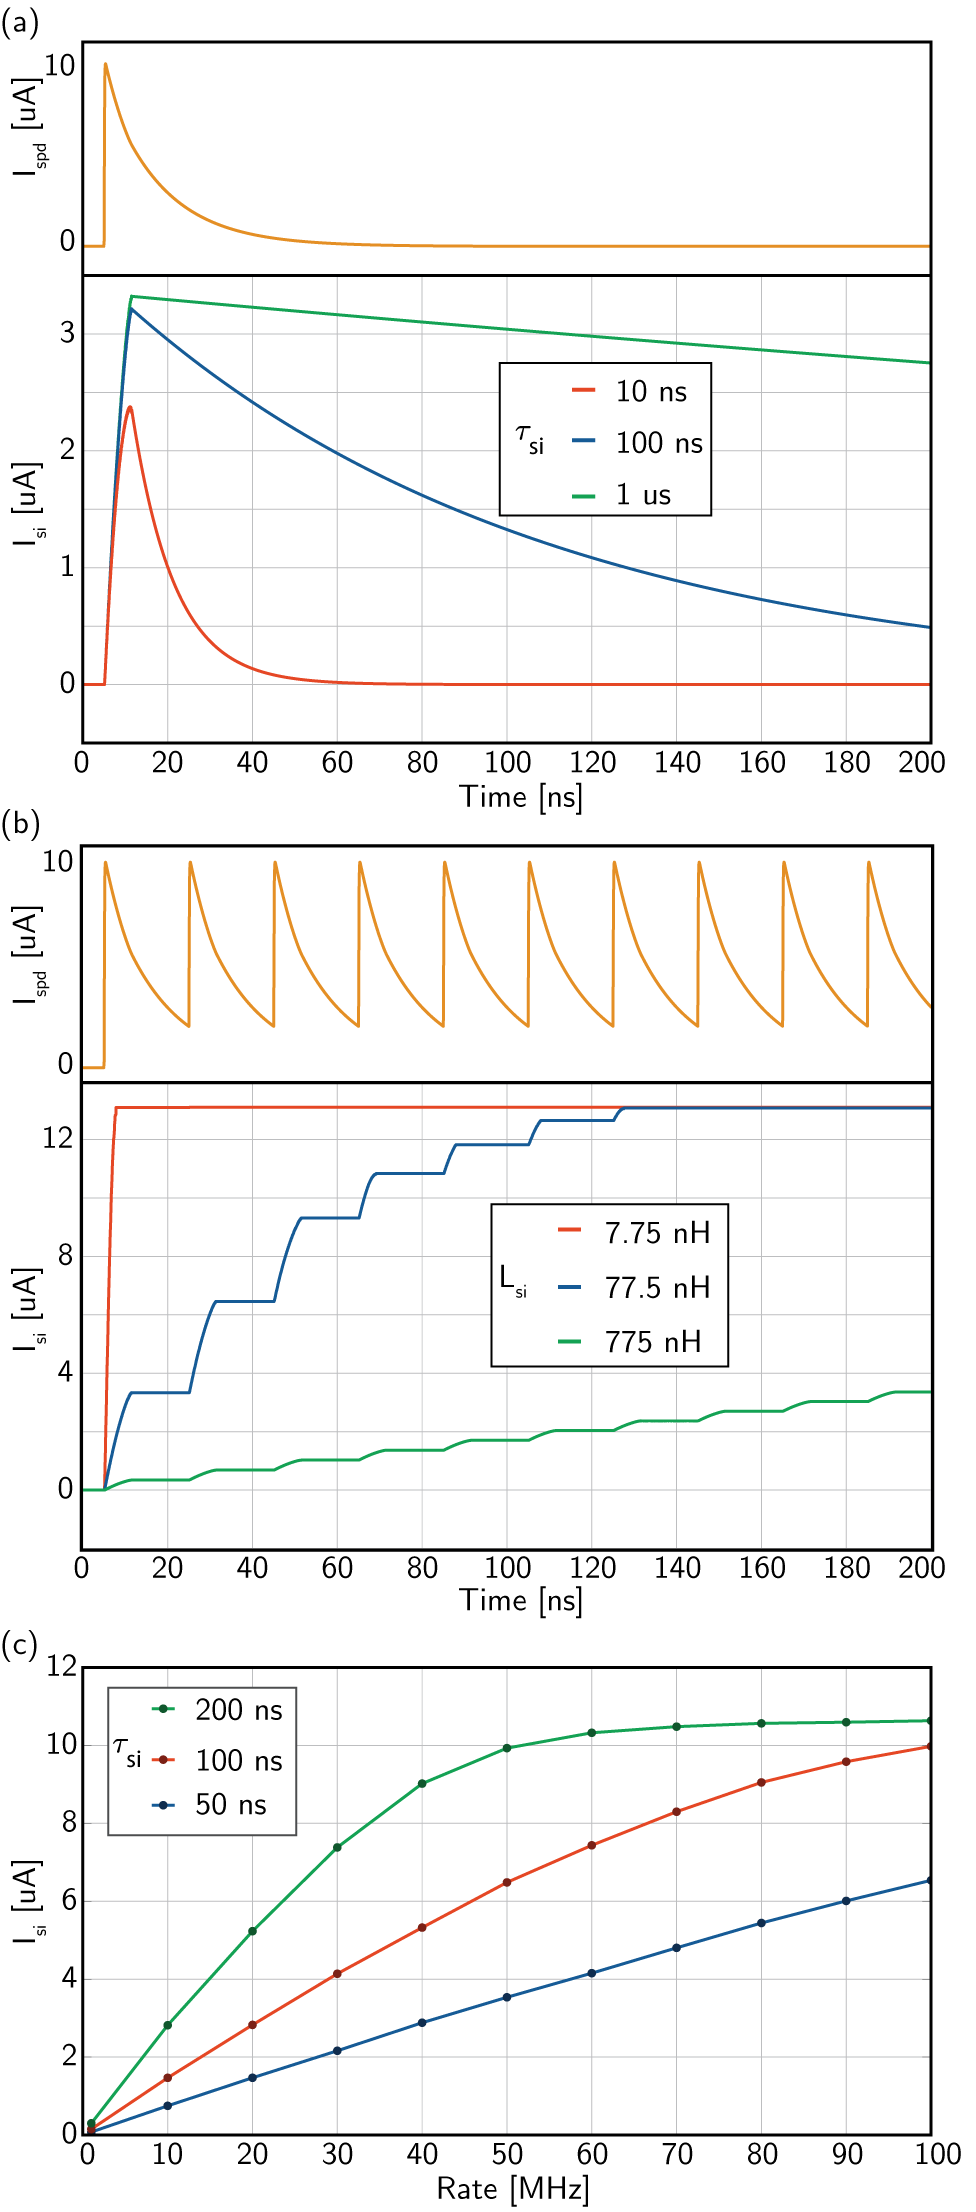
\includegraphics[width=8.6cm]{_3_sffg_temporal_functions.png}}
	\captionof{figure}{\label{fig:sffg}Caption.}
\end{figure}

\section{\label{sec:short_term}Operations on pulse trains at a single synapse}

\begin{figure} 
    \centering{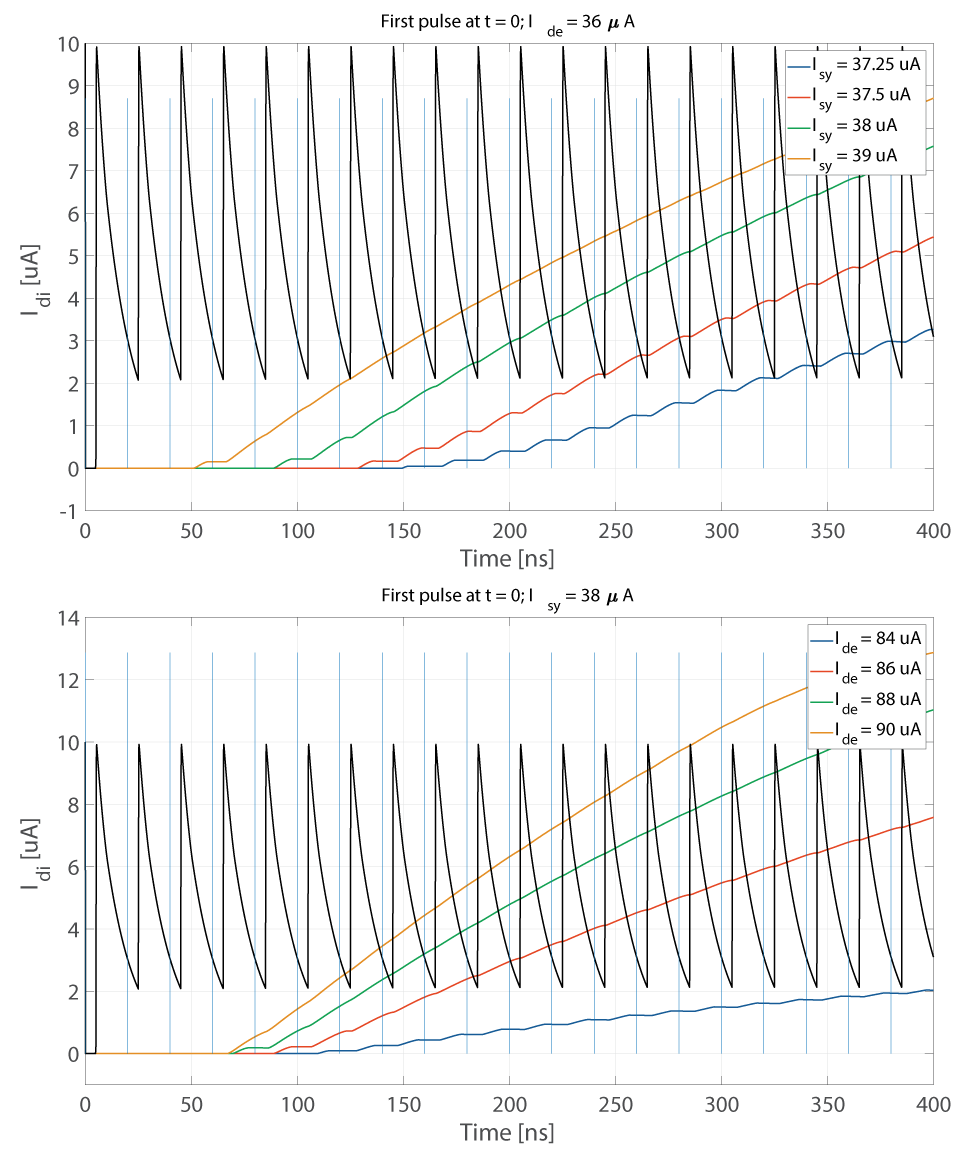
\includegraphics[width=8.6cm]{_4__si_di_facilitating.png}}
	\captionof{figure}{\label{fig:facilitating}Caption.}
\end{figure}

\begin{figure} 
    \centering{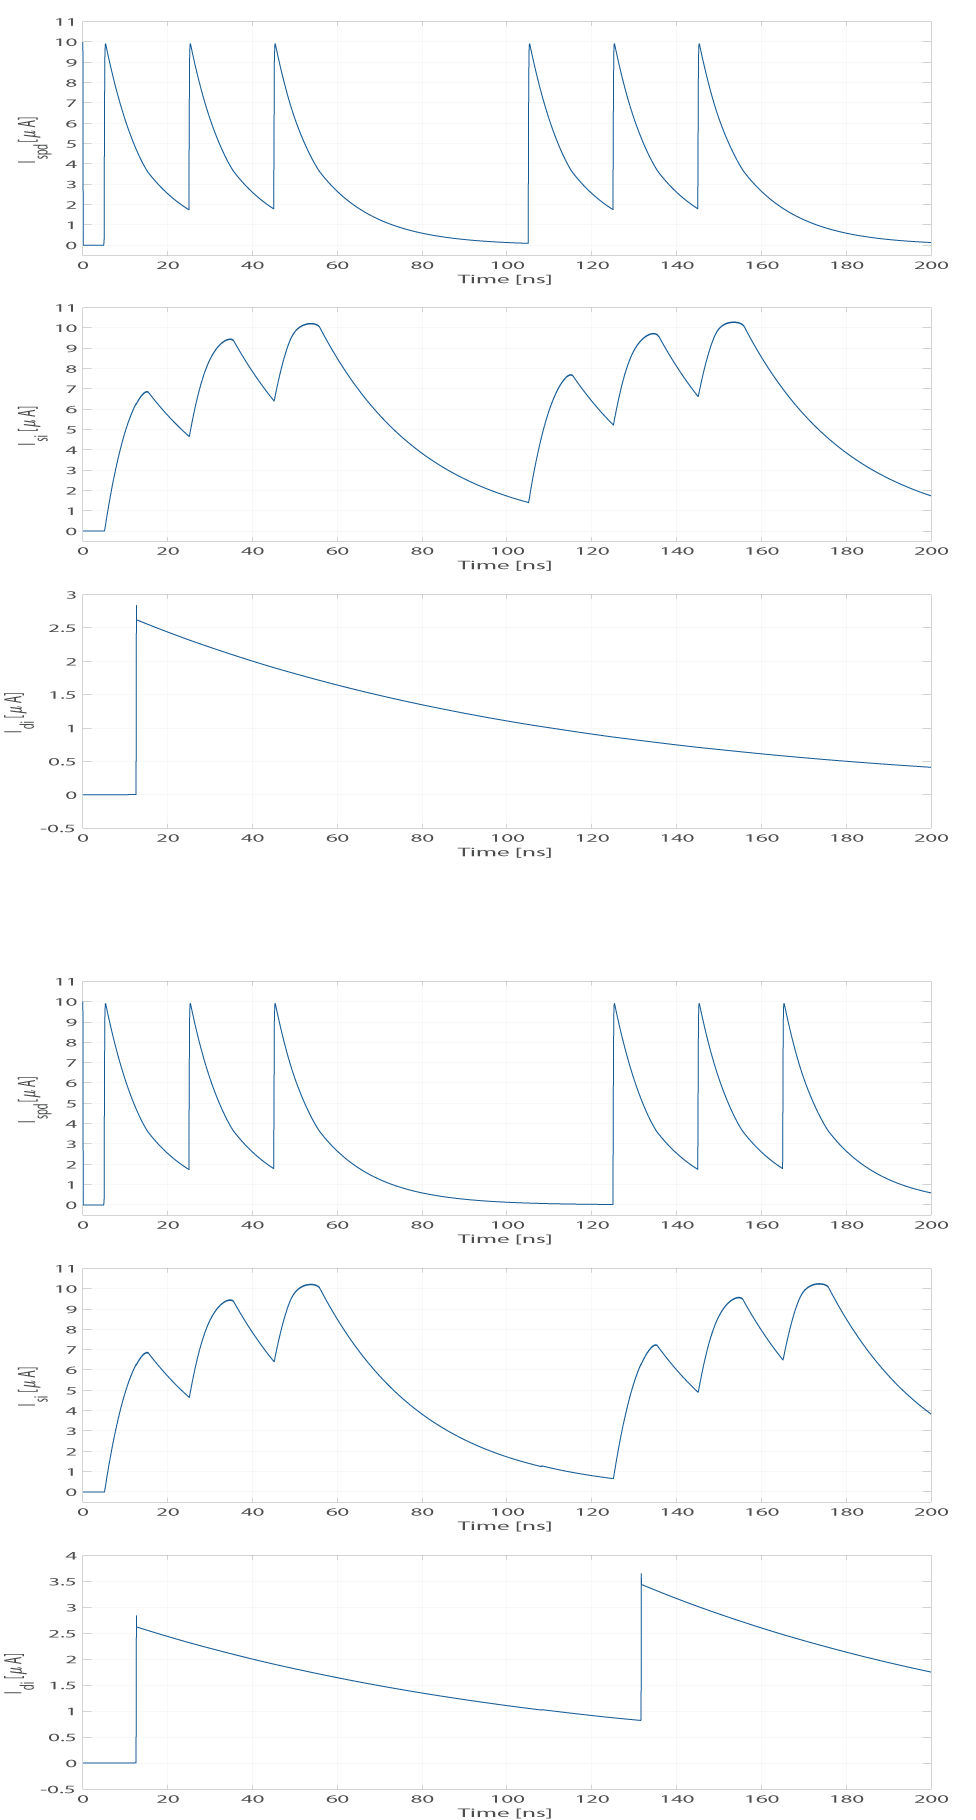
\includegraphics[width=8.6cm]{_5__si_dcsfq_depressing.png}}
	\captionof{figure}{\label{fig:depressing}Caption.}
\end{figure}

\section{\label{sec:correlations}Detecting correlations between neurons}

\begin{figure} 
    \centering{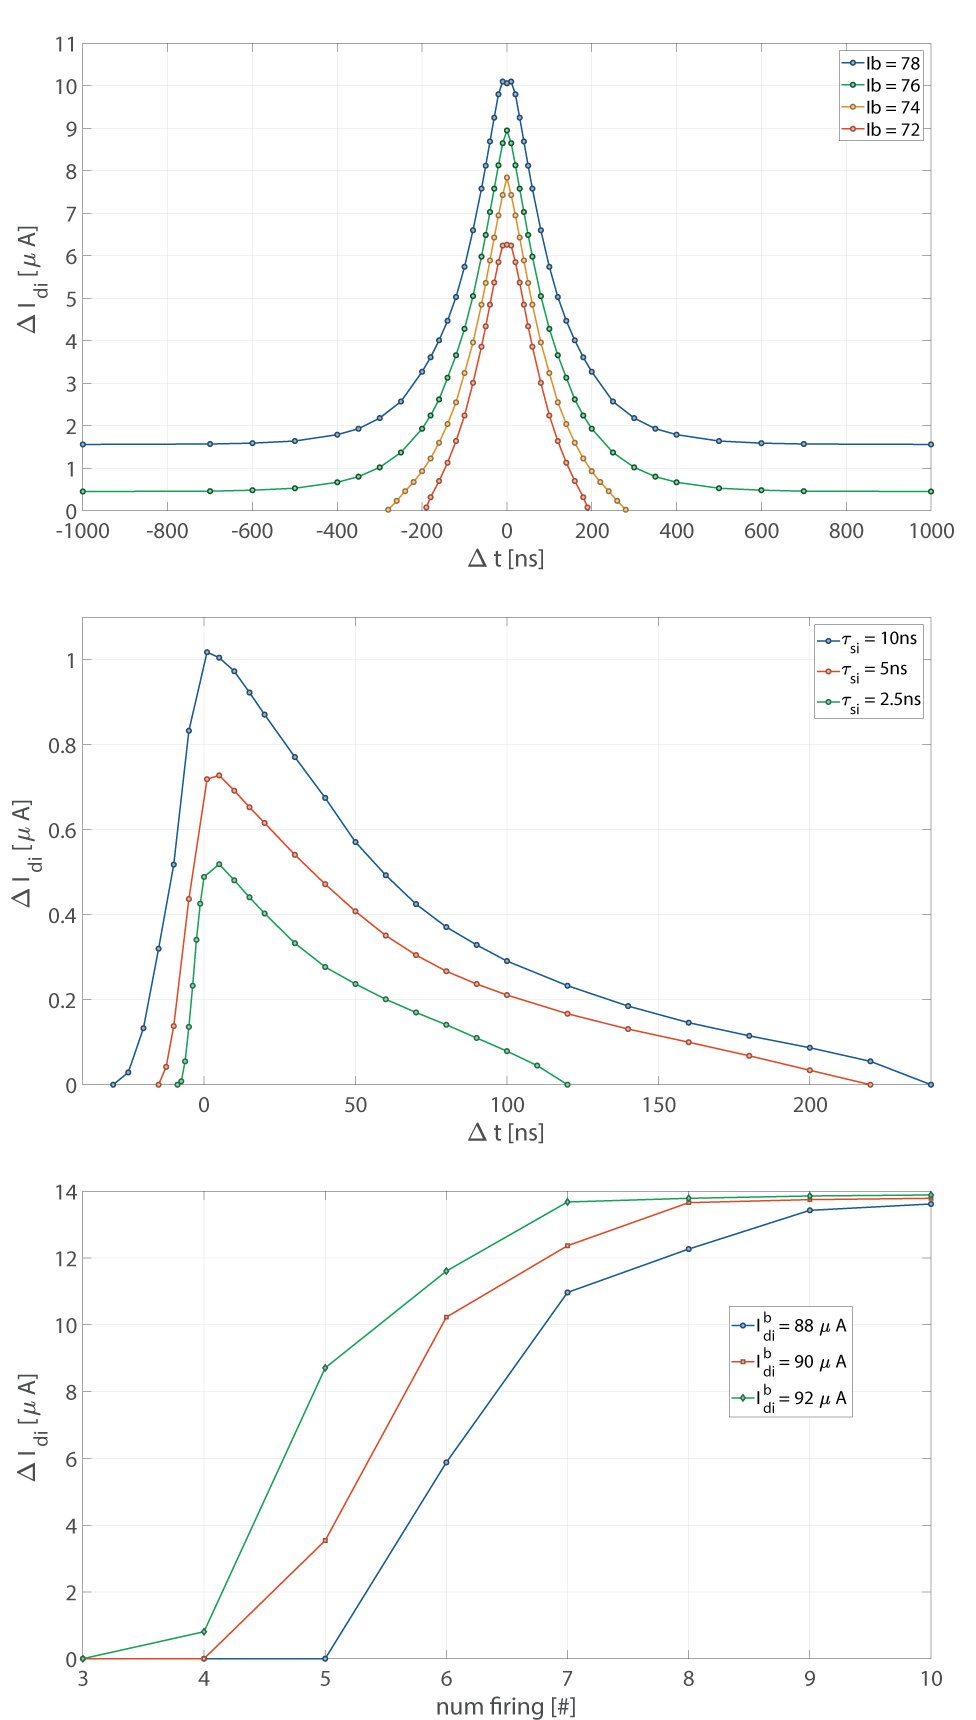
\includegraphics[width=8.6cm]{_6__poly_si_di.png}}
	\captionof{figure}{\label{fig:poly_si}Caption.}
\end{figure}

\section{\label{sec:inhibition_and_rapid_query}Inhibition and rapid query}

\begin{figure} 
    \centering{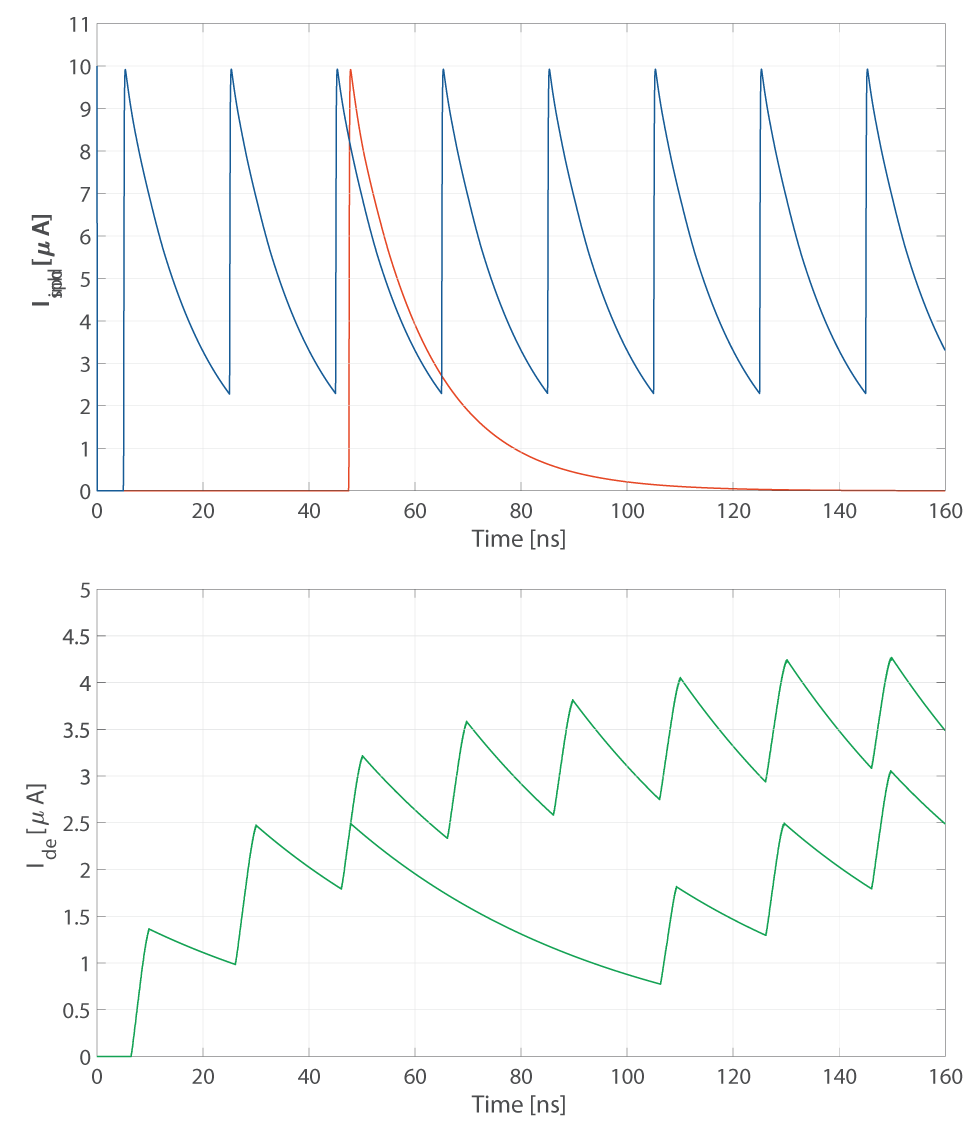
\includegraphics[width=8.6cm]{_7__si_di_inhibition.png}}
	\captionof{figure}{\label{fig:inhibition}Caption.}
\end{figure}

\begin{figure} 
    \centering{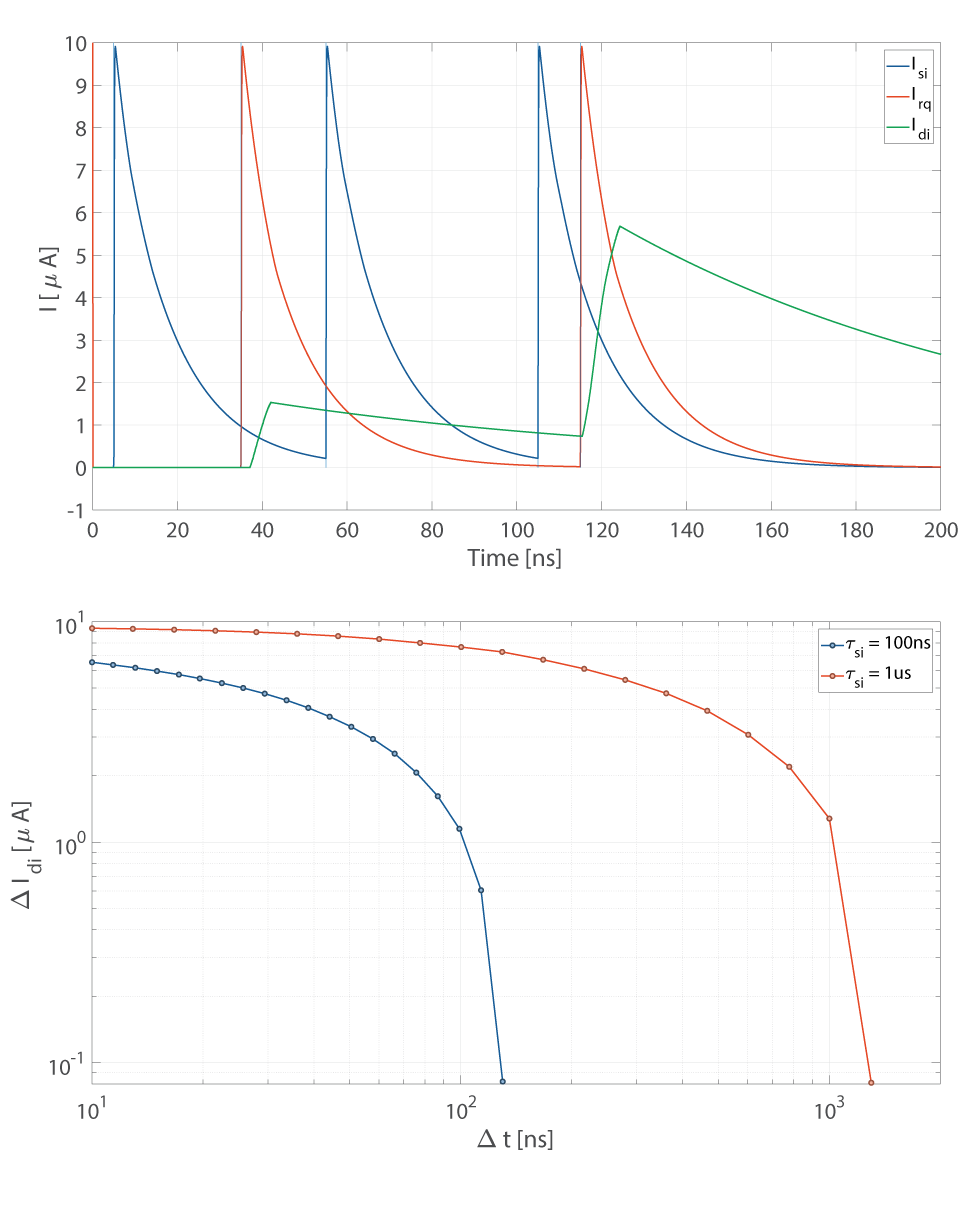
\includegraphics[width=8.6cm]{_8__si_di_rapid_query.png}}
	\captionof{figure}{\label{fig:inhibition}Caption.}
\end{figure}

\begin{figure} 
    \centering{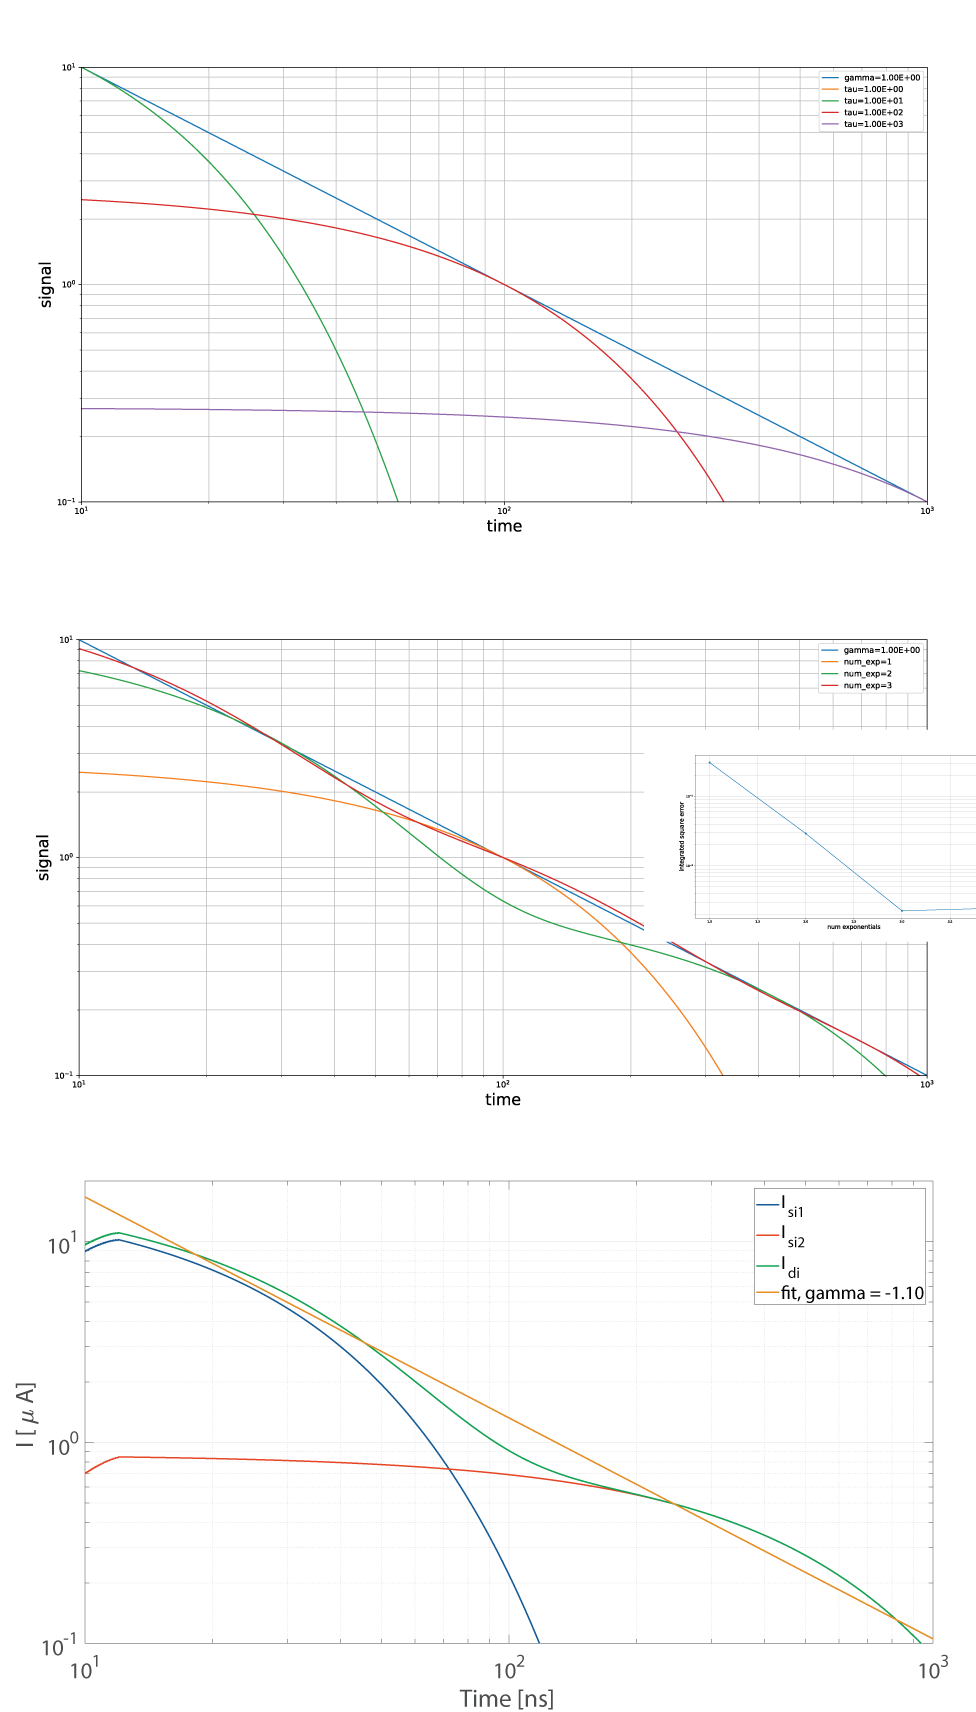
\includegraphics[width=8.6cm]{_9__power_law_time_decay.png}}
	\captionof{figure}{\label{fig:inhibition}Caption.}
\end{figure}

\section{\label{sec:fluxonic_fanout}Fanout to multiple synapses from the same neuron}

\section{\label{sec:discussion}Discussion}
	
\newpage
\appendix

\bibliographystyle{unsrt}
\bibliography{fluxonic_processing_of_photonic_synapse_events}

\end{document}